\documentclass[11pt]{article}
\usepackage[margin=0.9in]{geometry}
\usepackage{booktabs,longtable,array,amsmath,amssymb,xcolor,enumitem}
\usepackage{titlesec,fancyhdr,tabularx}
\usepackage[hidelinks]{hyperref}
\usepackage{tikz}
\usetikzlibrary{arrows.meta,positioning,fit,backgrounds}

\newcommand{\sig}[1]{\texttt{#1}}
\newcommand{\reg}[1]{\texttt{#1}}
\newcommand{\note}[1]{\par\smallskip\noindent\textit{Note:} #1\par}
\newcolumntype{L}[1]{>{\raggedright\arraybackslash}p{#1}}
\newcolumntype{C}[1]{>{\centering\arraybackslash}p{#1}}

\pagestyle{fancy}\fancyhf{}
\lhead{RMC — DFI\,$\rightleftarrows$\,Core Exchange Fabric}
\rhead{Block 01}\cfoot{\thepage}

\titleformat{\section}{\large\bfseries}{\thesection}{0.6em}{}
\titleformat{\subsection}{\normalsize\bfseries}{\thesubsection}{0.6em}{}

\begin{document}

\begin{center}
{\LARGE\bfseries DFI $\rightleftarrows$ MC-Core Exchange Fabric}\\[2pt]
{\large Register \& Buffer Enumeration --- Phase 1, Block 01}\\[6pt]
{\footnotesize Grounded in DFI 5.2 signal groups + RMC clock plan. Latencies programmable;
this doc fixes \emph{structure}.}
\end{center}
\vspace{4pt}\hrule\vspace{10pt}

%======================================================================
\section{Where it sits, what it does}

The exchange fabric is the boundary block between the MC scheduler core and the DFI port.
Everything the core hands the PHY, everything the PHY hands back, and every register that
configures, observes, or errors that exchange lives here.

\begin{center}
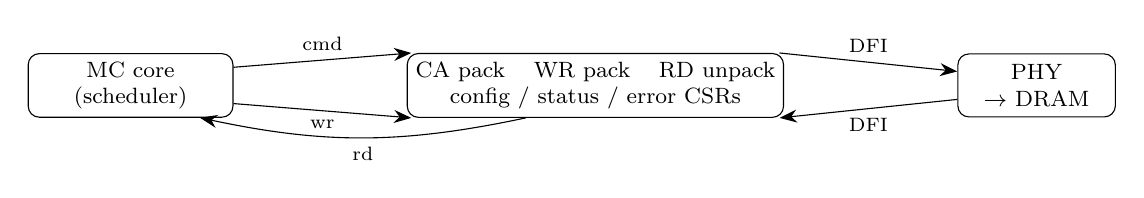
\begin{tikzpicture}[
  font=\footnotesize,
  blk/.style={draw,rounded corners,align=center,minimum height=8mm,inner sep=3pt},
  grp/.style={draw,dashed,rounded corners,inner sep=8pt},
  >={Stealth[length=2.2mm]}]
  \node[blk,minimum width=26mm] (core) {MC core\\(scheduler)};
  \node[blk,minimum width=40mm,right=22mm of core] (fab)
       {CA pack $\;\;$ WR pack $\;\;$ RD unpack\\ config / status / error CSRs};
  \node[blk,minimum width=20mm,right=22mm of fab] (phy) {PHY\\$\rightarrow$ DRAM};
  \draw[->] (core.10) -- node[above]{\scriptsize cmd} (fab.170);
  \draw[->] (core.-10) -- node[below]{\scriptsize wr} (fab.190);
  \draw[<-] (core.-25) to[bend right=12] node[below]{\scriptsize rd} (fab.205);
  \draw[->] (fab.10) -- node[above]{\scriptsize DFI} (phy.170);
  \draw[<-] (fab.-10) -- node[below]{\scriptsize DFI} (phy.190);
\end{tikzpicture}
\end{center}

\textbf{Three jobs:}
\begin{enumerate}[nosep,leftmargin=1.4em]
  \item \textbf{Serialize / deserialize} --- core speaks 1 command / 1 burst per
    transaction; DFI speaks \emph{phases} (\sig{dfi\_*\_pN}). Fabric packs core$\to$phases,
    unpacks phases$\to$core, per the gear ratio.
  \item \textbf{Cross clocks} --- core clock and DFI/PHY clock need not be edge-aligned.
    Data, command, and handshakes cross through CDC structures here.
  \item \textbf{Hold the CSRs} --- all DFI config, latency, status, update, and error state.
\end{enumerate}

%======================================================================
\section{Clock domains \& gear ratio}

\begin{center}\begin{tabular}{@{}lll@{}}\toprule
Domain & Clock & Runs \\ \midrule
\sig{core} & \sig{mc\_clk} & scheduler, queues, arbiter, scoreboard \\
\sig{dfi} & \sig{dfi\_clk} & DFI port I/O, phase pack/unpack \\ \bottomrule
\end{tabular}\end{center}

\begin{itemize}[nosep,leftmargin=1.4em]
  \item DRAM \sig{tCK} is faster still, PHY-internal. Fabric never sees \sig{tCK} directly ---
    the \textbf{gear ratio} abstracts it: 1 \sig{dfi\_clk} $=G$ \sig{tCK}.
  \item \sig{dfi\_freq\_ratio}: \textbf{1:1}$\to$G=1$\to$1 phase (\sig{\_p0});
    \textbf{1:2}$\to$G=2$\to$\sig{\_p0,\_p1}; \textbf{1:4}$\to$G=4$\to$\sig{\_p0..\_p3}.
  \item \textbf{Worst-case span $=$ 1:1\,\ldots\,1:4.} Buffers/packers parameterize on $G$:
    phase count $NPH=G$, data-word count $NW=G$ (word $=$ DQ$\times2$, double-edge packed).
  \item Baseline \sig{mc\_clk}$=$\sig{dfi\_clk}: CDC degenerates to a register stage --- CDC
    FIFOs stay parameterized (depth $\ge1$) so an async ratio is a config change, not a
    redesign.
\end{itemize}

%======================================================================
\section{Register classes (CSR map)}

Five classes. Address map is a later pass; here we fix \emph{what exists}.

\subsection{2A --- Static configuration (RW, set at init)}
\begin{center}\begin{tabular}{@{}lcL{8.4cm}@{}}\toprule
Reg & W & Meaning \\ \midrule
\reg{cfg\_freq\_ratio} & 2 & 00=1:1, 01=1:2, 10=1:4 (drives NPH/NW everywhere) \\
\reg{cfg\_2n\_mode} & 1 & 1=2N geardown on CA (DDR5 power-on default), 0=1N \\
\reg{cfg\_dram\_density} & 3 & 8/16/24/32\,Gb $\to$ bank count, tRFC select \\
\reg{cfg\_dq\_width} & 2 & x4/x8/x16 (DQ lanes, wrdata width, banks-per-BG halving) \\
\reg{cfg\_rank\_count} & 2 & ranks present ($\to$ \sig{dfi\_cs} fan, per-rank timing) \\
\reg{cfg\_bl\_mode} & 2 & BL16 / BL32 / BC8-OTF / BL16-OTF \\
\reg{cfg\_geardown\_en} & 1 & DDR5 1N/2N geardown enable mirror \\
\reg{cfg\_dbi\_wr\_en} & 1 & write DBI enable \\
\reg{cfg\_dbi\_rd\_en} & 1 & read DBI enable \\
\reg{cfg\_ca\_parity\_en} & 1 & CA parity generation enable \\
\reg{cfg\_wr\_crc\_en} & 1 & write CRC enable \\
\reg{cfg\_rd\_crc\_en} & 1 & read CRC check enable \\
\reg{cfg\_odt\_en} & 1 & ODT drive enable \\
\reg{cfg\_cs\_map} & N & logical rank $\to$ \sig{dfi\_cs} bit mapping \\ \bottomrule
\end{tabular}\end{center}

\subsection{2B --- Timing configuration (DFI 5.2 \sig{tphy\_*})}
All in \sig{dfi\_clk} cycles. These set the fabric pipe depths and the data-buffer
release/capture offsets.
\begin{center}\begin{tabular}{@{}lL{9.6cm}@{}}\toprule
Reg & Meaning \\ \midrule
\reg{t\_phy\_wrlat} & WR command $\to$ assert \sig{dfi\_wrdata\_en} (write launch offset) \\
\reg{t\_phy\_wrdata} & \sig{dfi\_wrdata\_en} $\to$ \sig{dfi\_wrdata} valid (data-vs-enable skew) \\
\reg{t\_phy\_rdlat} & RD command $\to$ \sig{dfi\_rddata} returns \\
\reg{t\_rddata\_en} & RD command $\to$ assert \sig{dfi\_rddata\_en} (read window open) \\
\reg{t\_phy\_wrcslat} & WR \sig{dfi\_wrdata\_cs} lead \\
\reg{t\_phy\_rdcslat} & RD \sig{dfi\_rddata\_cs} lead \\
\reg{t\_ctrl\_delay} & control-signal (CKE/ODT/\ldots) pipeline delay \\
\reg{t\_dram\_clk\_enable} & clock-enable assert $\to$ stable \\
\reg{t\_wrdata\_delay} & fabric-side write-data staging delay \\
\reg{t\_phy\_wrlvl\_*} & write-leveling latencies (training) \\
\reg{t\_phy\_rdlvl\_*} & read-leveling / gate-training latencies \\ \bottomrule
\end{tabular}\end{center}
\note{These are \emph{inputs} to buffer sizing: RD buffer depth $\ge$ \sig{t\_phy\_rdlat}
worth of outstanding phases; WR buffer holds data from enqueue until \sig{t\_phy\_wrlat}.}

\subsection{2C --- Live status (RO)}
\begin{center}\begin{tabular}{@{}lcL{8.2cm}@{}}\toprule
Reg & W & Meaning \\ \midrule
\reg{sts\_init\_complete} & 1 & \sig{dfi\_init\_complete} seen --- PHY/DRAM up \\
\reg{sts\_dram\_clk\_state} & 1 & DRAM clock enabled/disabled \\
\reg{sts\_wr\_buf\_level} & $\log_2$ & write-data buffer occupancy \\
\reg{sts\_rd\_buf\_level} & $\log_2$ & read-data buffer occupancy \\
\reg{sts\_ca\_buf\_level} & $\log_2$ & CA/command out buffer occupancy \\
\reg{sts\_wr\_cdc\_full} & 1 & write CDC FIFO full flag \\
\reg{sts\_rd\_cdc\_full} & 1 & read CDC FIFO full flag \\
\reg{sts\_lp\_state} & 2 & low-power handshake state \\
\reg{sts\_upd\_state} & 2 & ctrlupd/phyupd handshake state \\
\reg{sts\_training\_state} & 3 & current training phase \\
\reg{sts\_freq\_ratio\_now} & 2 & active gear ratio (post frequency-change) \\
\reg{sts\_ca\_quiesced} & 1 & CA path held for update/refresh (emit interlock) \\ \bottomrule
\end{tabular}\end{center}

\subsection{2D --- Update / handshake registers}
DFI has three update handshakes; fabric owns the MC side of each.
\begin{center}\begin{tabular}{@{}lL{5.2cm}L{5.2cm}@{}}\toprule
Handshake & DFI signals & Fabric reg \\ \midrule
Controller update & \sig{dfi\_ctrlupd\_req/\_ack} & \reg{upd\_ctrl\_req} (W1S), \reg{\_ack} (RO), \reg{\_interval} (RW) \\
PHY update & \sig{dfi\_phyupd\_req/\_ack/\_type} & \reg{upd\_phy\_req} (RO), \reg{\_ack} (W1S), \reg{\_type} (RO) \\
PHY master & \sig{dfi\_phymstr\_req/\_ack/\_state} & \reg{upd\_phymstr\_req} (RO), \reg{\_ack} (W1S), \reg{\_state} (RO) \\
Freq change & \sig{dfi\_freq\_ratio/\_fsp} & \reg{upd\_freq\_req} (W1S), \reg{\_ratio} (RW), \reg{\_ack} (RO) \\ \bottomrule
\end{tabular}\end{center}
\note{\textbf{Interlock:} a \sig{ctrlupd}/\sig{phyupd} in flight quiesces the CA path ---
\reg{sts\_ca\_quiesced} gates emit. This is the hook the refresh/maintenance path reads.}

\subsection{2E --- Error / interrupt registers (RO + W1C)}
\begin{center}\begin{tabular}{@{}lcL{8.2cm}@{}}\toprule
Reg & W & Meaning \\ \midrule
\reg{err\_dfi\_error} & 1 & \sig{dfi\_error} asserted (W1C) \\
\reg{err\_dfi\_error\_info} & N & captured \sig{dfi\_error\_info} code \\
\reg{err\_wr\_cdc\_ovf} & 1 & write CDC overflow (W1C) --- backpressure bug \\
\reg{err\_rd\_cdc\_ovf} & 1 & read CDC overflow (W1C) \\
\reg{err\_rddata\_timeout} & 1 & RD launched, no \sig{dfi\_rddata\_valid} in window (W1C) \\
\reg{err\_ca\_parity} & 1 & CA parity error reported by DRAM (W1C) \\
\reg{err\_wr\_crc} & 1 & write CRC error alert (W1C) \\
\reg{err\_rd\_crc} & 1 & read CRC mismatch (W1C) \\
\reg{err\_underrun\_wr} & 1 & \sig{dfi\_wrdata\_en} high but buffer empty (W1C) \\
\reg{err\_mask} & N & per-source interrupt mask (RW) \\
\reg{err\_status} & N & live OR of unmasked error bits (RO) $\to$ IRQ \\ \bottomrule
\end{tabular}\end{center}

%======================================================================
\section{Buffers (data-path)}

Three transfer buffers + their CDC crossings. All parameterized on $G$.

\subsection{3A --- CA / command out path (core $\to$ DFI)}
\begin{itemize}[nosep,leftmargin=1.4em]
  \item \textbf{Command out FIFO} --- emitted commands (opcode + bank/bg/row/col + CID +
    rank) waiting to be phased onto \sig{dfi\_address[13:0]} / \sig{dfi\_cs} / \sig{dfi\_act\_n}.
  \item \textbf{Phase packer} --- expands 1 command into CA phases: 1-cycle command
    (REF/PRE/MPC/powerdown/Vref) $\to$ 1 slot; 2-cycle command (ACT/RD/WR/WRP/MRW/MRR)
    $\to$ 2 slots (2N: 2nd half $+2$\,\sig{tCK}; 1N: adjacent). Maps slots onto
    \sig{\_p0..\_p(G-1)}; low-$G$ tail carries into next phase group.
  \item \textbf{CS/CKE/ODT driver} --- per-phase \sig{dfi\_cs/\_cke/\_odt/\_reset\_n},
    timed by \sig{t\_ctrl\_delay}. Plus CA parity gen if \reg{cfg\_ca\_parity\_en}.
  \item Depth shallow ($\ge NPH+$slack); CA budget 1 cmd / 2\,\sig{tCK}, never starves if
    scheduler respects \sig{caFree}.
\end{itemize}

\subsection{3B --- Write data out path (core $\to$ DFI)}
\begin{itemize}[nosep,leftmargin=1.4em]
  \item \textbf{Write-data buffer} --- holds full burst (BL16 $\to$ 16\,UI $\times$ DQ) + mask
    + optional DBI/CRC, from WR commit until \sig{t\_phy\_wrlat} after WR reaches CA. Core
    must hold data for the launch latency --- this buffer \emph{is} that hold. Entry $=$ one
    burst; depth $\ge \lceil$\sig{t\_phy\_wrlat}$/$burst-spacing$\rceil +$ margin. Width/phase
    $=$ \sig{dfi\_wrdata\_pN} $=$ DQ$\times2$; $NW=G$ words.
  \item \textbf{Write-mask lane} --- \sig{dfi\_wrdata\_mask} packed alongside.
  \item \textbf{WR data CDC FIFO} --- if async, burst crosses here (gray-pointer);
    \reg{sts\_wr\_cdc\_full} / \reg{err\_wr\_cdc\_ovf}.
  \item \textbf{Launch aligner} --- asserts \sig{dfi\_wrdata\_en} \sig{t\_phy\_wrlat} after WR,
    drives \sig{dfi\_wrdata} \sig{t\_phy\_wrdata} after enable; \sig{dfi\_wrdata\_cs} led by
    \sig{t\_phy\_wrcslat}.
  \item \textbf{Underrun guard} --- \reg{err\_underrun\_wr} if enable window opens on empty.
\end{itemize}

\subsection{3C --- Read data in path (DFI $\to$ core)}
\begin{itemize}[nosep,leftmargin=1.4em]
  \item \textbf{RD outstanding tracker} --- per launched RD: expected return slot, rank/CID,
    target queue entry, so returned phases route to the right requester. Sized $\ge$ commands
    in flight over \sig{t\_phy\_rdlat}.
  \item \textbf{Read-data capture buffer} --- captures \sig{dfi\_rddata\_pN} on
    \sig{dfi\_rddata\_valid} (\sig{t\_phy\_rdlat} after RD, window opened by
    \sig{dfi\_rddata\_en} at \sig{t\_rddata\_en}). \textbf{Phase unpacker} reassembles $G$
    words; DBI decode / CRC check as configured.
  \item \textbf{RD data CDC FIFO} --- crosses \sig{dfi\_clk}$\to$\sig{mc\_clk};
    \reg{sts\_rd\_cdc\_full} / \reg{err\_rd\_cdc\_ovf}.
  \item \textbf{Return router} --- hands reassembled burst + tag to the core read-return path.
  \item \textbf{Timeout guard} --- \reg{err\_rddata\_timeout} if valid never arrives.
\end{itemize}

%======================================================================
\section{CDC crossing structures}
\begin{center}\begin{tabular}{@{}lL{2.4cm}L{5.4cm}L{3.2cm}@{}}\toprule
Crossing & Direction & Structure & Flags \\ \midrule
Command & core$\to$dfi & gray-ptr async FIFO (or reg stage if sync) & \reg{sts\_ca\_buf\_level} \\
Write data & core$\to$dfi & async FIFO, burst-wide & \reg{sts\_wr\_cdc\_full}, \reg{err\_wr\_cdc\_ovf} \\
Read data & dfi$\to$core & async FIFO, burst-wide & \reg{sts\_rd\_cdc\_full}, \reg{err\_rd\_cdc\_ovf} \\
Handshakes & both & 2-flop synchronizers (req/ack) & per handshake \\
CSR access & core$\to$dfi & 2-flop sync on control bits & --- \\ \bottomrule
\end{tabular}\end{center}
\note{\textbf{Rule:} every multi-bit field crossing domains goes through a FIFO or is
captured on a single synchronized enable --- no bit-by-bit 2-flop on buses. Single-bit
control/status $\to$ 2-flop synchronizers; req/ack $\to$ 4-phase level protocol.}

%======================================================================
\section{Core-side contract (what the scheduler sees)}
Ports the scheduler talks to (names align later with \sig{RMC\_IO\_Map}):
\begin{center}\begin{tabular}{@{}lL{9.4cm}@{}}\toprule
Port & Meaning \\ \midrule
\sig{caFree} / \sig{ca\_credit} & from CA out FIFO: may I emit a command this cycle \\
\sig{wr\_data\_push} + \sig{wr\_data\_ready} & commit a write burst into the WR buffer \\
\sig{rd\_return} + \sig{rd\_tag} + \sig{rd\_return\_valid} & reassembled read burst back to core \\
\sig{maint\_quiesce} & (= \reg{sts\_ca\_quiesced}) update/refresh in flight, hold emit \\
\sig{init\_complete}, \sig{error\_irq} & bring-up + fault to the core control path \\ \bottomrule
\end{tabular}\end{center}
Everything else (phase packing, latencies, CDC, DFI signaling) is hidden behind this
contract. \emph{The scheduler schedules commands; the fabric makes them DFI phases.}

%======================================================================
\section*{Open items (fabric)}
\begin{description}[nosep,leftmargin=3.2em,style=nextline]
  \item[OF-1] exact CSR address map + access widths --- register-map pass.
  \item[OF-2] WR/RD buffer depths --- pin once \sig{t\_phy\_wrlat}/\sig{t\_phy\_rdlat} chosen.
  \item[OF-3] async vs synchronous baseline --- plan \sig{mc\_clk}$=$\sig{dfi\_clk}; confirm
    before sizing CDC FIFO depth.
  \item[OF-4] training-path detail (wrlvl/rdlvl/wdqlvl regs) --- enumerate in a sub-pass.
  \item[OF-5] CA parity / CRC error recovery policy --- replay vs report-only.
\end{description}

\end{document}
